\documentclass[a4paper,12pt]{report}

\usepackage{graphicx}
\usepackage{url}
\usepackage{amsmath}
\usepackage[utf8]{inputenc}
\usepackage[english]{babel}
\usepackage[pagestyles]{titlesec}
\usepackage{pgf}
\usepackage{tikz}
\usepackage[section]{placeins}
\usepackage{listings}
\usepackage{color}
\usepackage{seqsplit}
\usepackage{csquotes}
\usepackage{siunitx}

\usetikzlibrary{arrows,automata}
\usetikzlibrary{positioning}

\tikzset{
  state/.style={
    rectangle,
    rounded corners,
    draw=black,
    minimum height=2em,
    inner sep=1pt,
    text centered,
  },
}

\newpagestyle{mystyle}{
  \sethead{\chaptertitle}{}{}
  \setfoot{}{\thepage}{}}
\pagestyle{mystyle}
 
\setlength{\parindent}{1em}
\setlength{\parskip}{1em}
\graphicspath{ {images/} }

\pagenumbering{roman}

\def\code#1{\texttt{\seqsplit{#1}}}

\definecolor{pblack}{rgb}{0.0,0.0,0.0}
\definecolor{pblue}{rgb}{0.0,0.0,0.5}
\definecolor{pbrightblue}{rgb}{0.0,0.0,1.0}
\definecolor{pgreen}{rgb}{0,0.5,0}
\definecolor{pred}{rgb}{0.9,0,0}
\definecolor{pgrey}{rgb}{0.5,0.5,0.5}
\definecolor{pdarkyellow}{rgb}{0.5,0.5,0.0}
\definecolor{ppurple}{rgb}{0.4,0.05,0.48}

\lstset{
  language            = Java,
  basicstyle          = \scriptsize,
  % xleftmargin         = -4.0em,
  % xrightmargin        = -4.0em,
  frame               = single,
  identifierstyle     = \color{pblack},
  commentstyle        = \color{pgrey},
  keywordstyle        = \color{pblue},
  stringstyle         = \color{pgreen},
  moredelim=[il][\textcolor{pdarkyellow}]{$$},
  moredelim=[is][\textcolor{pdarkyellow}]{\%\%}{\%\%}
}

\newcommand\JSONnumbervaluestyle{\color{pbrightblue}}
\newcommand\JSONstringkeystyle{\color{ppurple}}
\newcommand\JSONstringvaluestyle{\color{pgreen}}

\newif\ifcolonfoundonthisline
\newif\ifsquarebracketopen

\makeatletter

\lstdefinestyle{json}
{
  basicstyle          = \scriptsize,
  % xleftmargin         = -4.0em,
  % xrightmargin        = -4.0em,
  frame               = single,
  showstringspaces    = false,
  keywords            = {false,true},
  alsoletter          = 0123456789.,
  morestring          = [s]{"}{"},
  stringstyle         = \ifcolonfoundonthisline\JSONstringvaluestyle\else\ifsquarebracketopen\JSONstringvaluestyle\else\JSONstringkeystyle\fi\fi,
  MoreSelectCharTable =%
    \lst@DefSaveDef{`:}\colon@json{\processColon@json}
    \lst@DefSaveDef{`[}\squareBracketOpen@json{\processOpenSquareBracket@json}
    \lst@DefSaveDef{`]}\squareBracketClose@json{\processCloseSquareBracket@json},
  keywordstyle        = \color{pblue},
}

\newcommand\processColon@json{%
  \colon@json%
  \ifnum\lst@mode=\lst@Pmode%
    \global\colonfoundonthislinetrue%
  \fi
}

\newcommand\processOpenSquareBracket@json{%
  \squareBracketOpen@json%
  \ifnum\lst@mode=\lst@Pmode%
    \global\squarebracketopentrue%
  \fi
}

\newcommand\processCloseSquareBracket@json{%
  \squareBracketClose@json%
  \ifnum\lst@mode=\lst@Pmode%
    \global\squarebracketopenfalse%
  \fi
}

\lst@AddToHook{Output}{%
  \ifcolonfoundonthisline%
    \ifnum\lst@mode=\lst@Pmode%
      \def\lst@thestyle{\JSONnumbervaluestyle}%
    \fi
  \fi
  %override by keyword style if a keyword is detected!
  \lsthk@DetectKeywords% 
}

% reset the switch at the end of line
\lst@AddToHook{EOL}%
  {\global\colonfoundonthislinefalse}

\makeatother

\begin{document}

% Front matter
\begin{titlepage}
  \begin{center}
    {\LARGE Fast and precise automated analysis of algorithms' time complexity \par}
    \vskip 10.0em
                                                    		
    {\large
      \lineskip 1.0em
      \begin{tabular}[t]{c}
        Dario Simonetti \\Kellogg College\\University of Oxford
      \end{tabular}\par
    }
    \vskip 2.0em
                                                    		
    {\large 3rd of November 2017}
    \vskip 2.0em
                                                    		
    Supervised by: Anthony Widjaja Lin
    \vspace*{\fill}
                                                    		
    {
      
\includegraphics[width=5.0em,keepaspectratio]{oxford-logo.png}
      \vskip 1.0em
      A dissertation submitted in partial fulfilment of the requirements for the degree of Master of Science in Software Engineering
    }
  \end{center}
\end{titlepage}

\begin{abstract}
  Profilers have been around in the field of software development since the 70’s
  and have been – and still are – very useful in diagnosing problems and as tools
  for programs optimisation. They can analyse how much time the program is
  spending in each method. Based on this information the developer is able to
  detect what part of the program is taking more time than expected to execute and
  can act to improve it.
          
          
  What profilers can’t do is to estimate how much time it would take when the input
  size is increased. This dissertation supports the development of a tool that will
  estimate the time complexity of an algorithm under test with a high precision. This
  allows accurately estimating the time needed for the algorithm to solve a problem
  for any input size, giving developers a precise idea of how the software will
  behave with input sizes that haven’t been profiled.
\end{abstract}

\vspace*{\fill}
\noindent \textbf{Declaration}

\noindent The author confirms that: this dissertation does not contain material previously submitted for another degree or academic award; and the work presented here is the author's own, except where otherwise stated.

\tableofcontents

\pagenumbering{arabic} % Switch to normal numbers

% Main matter
\chapter{Introduction}
TODO
\chapter{Requirements analysis}

This chapter aims to determine the software requirements, so that these can be used for the design and consequently the implementation of the software.

\noindent The software can be divided into two different concerns: profiling and analysis. The profiling part is responsible for the measuring of time spent in each instrumented method. The analysis part takes the data measured by the profiler and works out the time complexity of the algorithm under test. These two concerns have very different types of requirements, mainly because the former runs at the same time as the tested algorithm, while the latter doesn't.

\section{Profiling}

\subsection{Limited observer effect impact}
As the profiler runs together with the algorithm under test, extra care needs to be taken in order to not be affected by the observer effect \cite{MSH08}. Because they are sharing the same CPU it is not possible to avoid the observer effect, but several things can be done in order to limit its impact as well as measuring it.

\subsection{Manual methods selection}
Often there are methods that are called very frequently and are very quick (e.g. getters and setters) and for this reason there needs to be a way of specifying which methods should be profiled and which ones shouldn't.

\noindent It should also allow to profile 3rd party code as it is sometimes useful to see when a lot of time is spent in a library that there is no control over, so that it can be potentially be swapped out for a different or a custom-built one. This will also allow to profile and analyse code that is part of the Java SDK, such as sorting and searching algorithms.

\noindent Method selection should be possible via Java annotations in the algorithm under test as well as by specifying whitelists and blacklists of methods' fully qualified names.

\subsection{Storage}
The profiler needs to be able to handle and store a vast number of measurements without running out of memory and space on disk.


TODO: add more?

\section{Analysis}

\subsection{Custom test}
As the software doesn't perform any static analysis of the algorithm under test, it does not know how to make sure to test all the edge cases. Moreover it doesn't know whether the edge cases are an important factor for the user who is analysing the algorithm (end user). \noindent For example, when measuring a sorting algorithm it might be important for the end user to know how well it performs under specific circumstances such as when the list is already ordered or ordered in decreasing order; it might be completely irrelevant too.

\noindent For these reasons, the test that is run by the profiler for each \emph{n} must be defined by the end user.

\subsection{Configuration}
It needs to be possible to easily change the analysis configuration in order to find the right balance between speed and accuracy:
\begin{itemize}
  \item \textbf{Max \emph{n}}: maximum value of \emph{n} to test the algorithm with
  \item \textbf{Number of samples per round}: number of samples to collect between $n = 1$ and $n = maxN$
  \item \textbf{Samples distribution}: how to distribute the samples in each round (linearly or exponentially).
  \item \textbf{Number of rounds per \emph{n}}: number of times to test the algorithm for each \emph{n}N
  \item \textbf{Number of warmup rounds per \emph{n}}: number of times to run the algorithm without measuring for each \emph{n}
  \item \textbf{Number of max outliers to exclude}: maximum number of out outliers to remove for each \emph{n}
\end{itemize}


\subsection{Supported curves}
Because the software analyses the methods in isolation, it only needs to fit the measured data to one of the basic "primitives" (TODO: is this really a requirement?):
\begin{itemize}
  \item Constant ($f(n) = a$)
  \item Linear ($f(n) = a \cdot n + b$)
  \item Quadratic ($f(n) = a \cdot n^2 + b \cdot n + c$)
  \item Cubic ($f(n) = a \cdot n^3 + b \cdot n^2 + c \cdot n + d$)
  \item Logarithmic ($f(n) = a \cdot log(n) + b$)
  \item Linearithmic ($f(n) = a \cdot n \cdot log(n) + b$)
  \item Exponential ($f(n) = a \cdot e^{(n \cdot b)} + c$)
\end{itemize}


TODO: add more?
\chapter{Design}

The purpose of this chapter is to describe how the software is designed based on the requirements specified in the previous chapter. Section \ref{sec:design:overview} gives a design overview and introduce the concept of module and the motivations for adopting this structure. Sections \ref{sec:design:annotations}-\ref{sec:design:timecomplexityanalyser} will each describe one of the modules that make up the whole software.

% TODO: why Java? Comfortable with it, easy instrumentation, generics, Akka, compatible with Scala (maybe not in this chapter)

\section{Overview}
\label{sec:design:overview}
The software will take a dynamic approach to determine the time complexity of the algorithm under test. The algorithm will be run with inputs of different size $n$, while at the same time recording how long is spent in each measured method and how many times each measured method is called.

\noindent Only the methods the end user thinks are relevant are measured and for each one of them their time complexity is calculated. The assumption that the dissertation tries to verify is that measuring the time complexity method by method is faster and potentially more accurate than measuring the whole algorithm. It's then trivial to work out the time complexity of the whole algorithm based on the time complexity of the measured methods that compose it.

\noindent In order to ensure low coupling and high cohesion \cite{EYC79}, the software will be divided in different modules, each one with a different responsibility. Classes within each module will honour the same principles. This will bring several advantages:
\begin{itemize}
  \item \textbf{Encouraged refactoring}: modules and classes can be refactored and optimised without impacting the rest of the code. This will encourage perfecting the code to keep it clean and maintainable
  \item \textbf{Increased reusability}: as each module and class is built to only do one job well (Single Responsibility Principle \cite{RCM03}), it is easy to reuse it for different applications
  \item \textbf{Improved robustness}: when the cohesion is high the code complexity is much lower, making it much easier to test
  \item \textbf{Reduced code duplication}: instead of defining logic more than once, it is coded once and used several time across the product (Don't Repeat Yourself \cite{AHT99}). Any changes in the logic would only have to be implemented in one single place
\end{itemize}

\noindent Figure \ref{fig:modules} shows an overview of the modules and the dependencies within them. The next chapters describe the modules shown in the diagram.

\begin{figure}
  \centering
  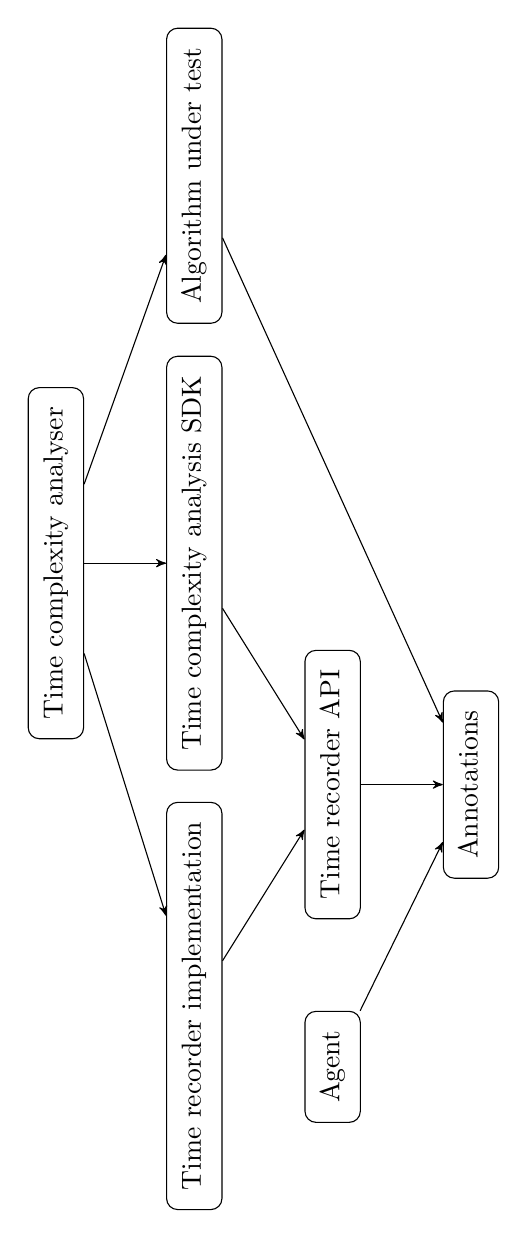
\begin{tikzpicture}[->,>=stealth', rotate=90, transform shape]
    % FIRST LAYER
    \node[state] (TIME_COMPLEXITY_ANALYSER) 
    {
      \begin{tabular}{c}
        Time complexity analyser 
      \end{tabular}
    };
              
    % SECOND LAYER
    \node[state,
      node distance=5.0em,
      below of=TIME_COMPLEXITY_ANALYSER] (TIME_COMPLEXITY_ANALYSIS_SDK) 
    {
      \begin{tabular}{c}
        Time complexity analysis SDK 
      \end{tabular}
    };
              
    \node[state,
      node distance=14.0em,
      left of=TIME_COMPLEXITY_ANALYSIS_SDK,
      xshift=-2.0em] (TIME_RECORDER_IMPL) 
    {
      \begin{tabular}{c}
        Time recorder implementation 
      \end{tabular}
    };
              
    \node[state,
      node distance=14.0em,
      right of=TIME_COMPLEXITY_ANALYSIS_SDK] (TEST_ALGORITHM) 
    {
      \begin{tabular}{c}
        Algorithm under test 
      \end{tabular}
    };
              
    % THIRD LAYER
    \node[state,
      node distance=5.0em,
      below of=TIME_RECORDER_IMPL,
      xshift=-2.2em] (AGENT) 
    {
      \begin{tabular}{c}
        Agent 
      \end{tabular}
    };
            
    \node[state,
      node distance=5.0em,
      below of=TIME_RECORDER_IMPL,
      xshift=+8.0em] (TIME_RECORDER_API) 
    {
      \begin{tabular}{c}
        Time recorder API 
      \end{tabular}
    };
              
    % FOURTH LAYER
    \node[state,
      node distance=5.0em,
      below of=TIME_RECORDER_API] (ANNOTATIONS) 
    {
      \begin{tabular}{c}
        Annotations 
      \end{tabular}
    };
            
    % LINES
    \path 
    (TIME_COMPLEXITY_ANALYSER) edge (TIME_RECORDER_IMPL)
    (TIME_COMPLEXITY_ANALYSER) edge (TIME_COMPLEXITY_ANALYSIS_SDK)
    (TIME_COMPLEXITY_ANALYSER) edge (TEST_ALGORITHM)
    (TIME_RECORDER_IMPL) edge (TIME_RECORDER_API)
    (TIME_COMPLEXITY_ANALYSIS_SDK) edge (TIME_RECORDER_API)
    (TEST_ALGORITHM) edge (ANNOTATIONS)
    (TIME_RECORDER_API) edge (ANNOTATIONS)
    (AGENT) edge (ANNOTATIONS)
    ;
  \end{tikzpicture}
  \caption{Modules overview}
  \label{fig:modules}
\end{figure}

\section{Annotations}
\label{sec:design:annotations}
This module doesn't contain any implementation, only Java annotations. A Java annotation is a special syntax used to associate metadata to packages, classes, methods, parameters and variables. They can be read and interpreted by the compiler at compile time or by an agent at runtime. These annotations are used to inform the agent (see next section) about what methods to instrument and measure.


\section{Agent}
\label{sec:design:agent}
This module contains the logic to instrument the algorithm under test. First the agent will detect which methods need to be instrumented based on annotations, whitelists and blacklists. Secondly the agent will instrument each of these methods by measuring the time passed during the method execution. This information will then be passed to the time recorder implementation (see next sections) which will take care of storing it for later processing.

\noindent The built agent is a JAR\footnote{https://docs.oracle.com/javase/8/docs/technotes/guides/jar/jarGuide.html} file which will need to be attached to the system by passing \code{-javaagent:jarpath[=options]}\footnote{https://docs.oracle.com/javase/8/docs/api/java/lang/instrument/package-summary.html} on the command-line, where \code{jarpath} is the path to the agent JAR while \code{options} are the options, such as whitelists and blacklists. This will instrument the algorithm under test at runtime when the instrumented methods are used for the first time.


\section{Time recorder API}
This module defines the API needed for time recording. The API will need to provide the interface for three different features:
\begin{itemize}
  \item \textbf{Start}: used by the system just before the algorithm's time complexity is about to be measured. This will reset any existing data in the time recorder implementation and start a fresh new recording
  \item \textbf{Report time}: used by the agent when an instrumented has just finished running to inform the time recorder implementation about how long it took. The implementation will take care of storing this information for later processing
  \item \textbf{Stop}: used by the system just after the algorithm is done running. This will shut down the time recorder implementation and return all the recorded data
\end{itemize}

\noindent Once all the rounds have run, the recorded data is processed and returned in form of a raw call tree.

\noindent Defining an API for time recording will keep the interface separated from the implementation so that the whole system works without needing to know the inner workings of the time recorder implementation. This allows easily swapping and comparing different implementations, which will be very useful in order to fine-tune them. On top of that developers can easily attempt building their own implementation in order to improve the existing one or to fine tune it for their specific use case. Because the implementation is probably the most delicate part of the whole system (as it needs to be accurate while ensuring a limited observer effect), being able to change the implementation must be an easy task.

\section{Time recorder implementation}
This module implements the time recorder API described in the previous section. The implementation needs to ensure that the act of recording doesn't have an impact on the actual measurement of the algorithm under test (i.e. limited observer effect). Time recording is purposely kept separate from the time complexity analysis as the former is run together with the algorithm under test while the latter isn't. In order to limit the observer effect is then essential to keep the CPU load as low as possible while the algorithm under test is running. 

\noindent This implementation is only responsible for storing the measured data for later retrieval and processing, which is something that doesn't put a big workload on the CPU. Had the time complexity be analysised as the algorithm under test was running, the measured time complexity would likely be far less accurate as the analysis is computationally expensive (see next sections).

\section{Time complexity analysis SDK}
This module is responsible for analysing the data captured by the time recorder. It does so in 7 different steps:
\begin{enumerate}
  \item \textbf{Warm-up}: run some rounds and ignore the recorded data. This will instrument all the methods that need to be measured, which will make the algorithm under test run slightly slower. The end user will be able to choose how many warm-up rounds to have (could be zero)
  \item \textbf{Record}: run the recording rounds. The rounds are run with different $n$ and each will produce a raw call tree measured by the time recorder. The end user will be able to choose what $n$'s to use and how many rounds to run for each $n$
  \item \textbf{Sequence}: each round that has run now has a corresponding raw call tree. Sequencing will take all the rounds for a specific $n$ and generate a single tree with a list of measurements in each node
  \item \textbf{Clean Up}: there are now several measurements in each node in each raw call tree, some of which are far from the average for that node (outliers) and are removed in this step. The end user will be able to choose the upper limit of how many outliers to exclude (could be zero)
  \item \textbf{Average}:  the remaining measurements in each node are averaged together so that there is only one value per node in each call tree
  \item \textbf{Normalise}: each node in the raw call tree now contains a measurement, which contains information about how many times it has been called and how much total time has been spent inside that method. Because of the simple nature of the time recorder, each node is affected by other nodes in the same tree branch. The number of times it has been called is affected by the number of times its parent has been called while the time spent inside the method is affected by the time spent in its children too. The normalisation process takes the call tree in raw format (see Figure \ref{fig:rawcalltree}) and ensures that each node only contains data related to that specific node (see Figure \ref{fig:normalisedcalltree})
  \item \textbf{Aggregate}: for each $n$ there is now one normalised call tree. The aggregation will take these trees and generate a single tree with a map in each node. The map keys represent $n$ while the values represent the normalised measurement for the corresponding key
  \item \textbf{Interpolate}: interpolation is the act of finding a curve that best approximates the relationship between $n$ and the corresponding normalised measurement, i.e. a function $f(n)$ that takes $n$ as input and returns the measurement as output (see example in Figure \ref{fig:interpolatedcalltree}). This function accurately describes the time complexity of the corresponding method in that specific call path (i.e. tree branch)
  \item \textbf{Calculate time complexity}: there is now one single call tree with a function $f(n)$ per node approximating the measurement of the corresponding method as a function of $n$. The time complexity can be calculated, describing the whole algorithm as a function of $n$ by simply navigating through the tree
\end{enumerate}

\noindent Once the time complexity function is determined, accurately calculating how long the algorithm would take to run given an input size $n$ can be done in constant time as it's a simple calculation.

\noindent Being an SDK, this module provides the tools for performing the analysis of an algorithm but won't do any of the above until correctly configured. For this reason this module has  has no dependency on the time recorder implementation and instead the code is done against the time recorder API. The time recorder implementation will be supplied at runtime and the whole wiring will be done by the time complexity analyser module (see next sections). Also it has no dependency on the algorithm under test and instead defines an interface describing an algorithm, which the algorithm under test will implement at runtime (see next chapter).

\noindent The SDK parameters specified above allow the end user to tweak the analysis to favour accuracy over speed and vice versa. The more rounds are run and the more accurate the time complexity will be and the slower it will be to calculate it.

\section{Algorithm under test}
This is the algorithm that is under test and that will be analysed. It can have a dependency on the annotations module, in case it wants to specify what methods to measure by using the provided annotations.

\section{Time complexity analyser}
\label{sec:design:timecomplexityanalyser}
This module puts everything together. It takes the time recording implementation and the algorithm under test and then uses the time complexity analysis SDK to calculate the algorithm's time complexity. This is where the end user can tweak the analysis by changing what SDK parameters, what time recorder implementation to use and what test to run for each round and each given $n$.
\chapter{Implementation}

TODO: intro

% Discuss requirements... measure observer effect
% Discuss precision and speed
% Maven

\section{Overview}

TODO


\section{Annotations}
\begin{lstlisting}
public @interface Measured {
}
\end{lstlisting}

\section{Agent}

TODO


\section{Time recorder API}

TODO


\section{Time recorder implementation}

TODO


\section{Time complexity analysis SDK}

TODO


\section{Algorithm under test}

TODO


\section{Time complexity analyser}

TODO

\chapter{Case studies}

\section{Overview}
\label{sec:casestudies:overview}
TODO by 25/09

\section{First}

TODO by 28/08


\section{Second}

TODO by 25/09
\chapter{Conclusion}
TODO by 16/10

% Back matter
\chapter{Bibliography}
\begin{thebibliography}{9}

\bibitem{MSH08}
  Todd Mytkowicz, Peter Sweeney, Matthias Hauswirth and Amer Diwan,
  \emph{Observer Effect and Measurement Bias in Performance Analysis},
  \url{http://scholar.colorado.edu/csci_techreports/972},
  Computer Science Technical Reports. Paper 972,
  2008.


\end{thebibliography}
\chapter{Appendices}
TODO


\end{document}
